\documentclass{standalone}
\usepackage{tikz}
\usepackage{pgfplots}
\pgfplotsset{compat=newest}
\usepackage{pgfmath}
\usepackage{tikz-cd}
\usepackage{pgffor}
\usepackage{tkz-euclide}
\usetkzobj{all}
\usepgfplotslibrary{fillbetween}
\usetikzlibrary{
	calc,
	angles,
	quotes,
	arrows.meta,
	decorations.markings,
	math,
	backgrounds,
	pgfplots.statistics,
	matrix,
	patterns,
	shapes.geometric,
	spy,
	intersections,
}
\begin{document}
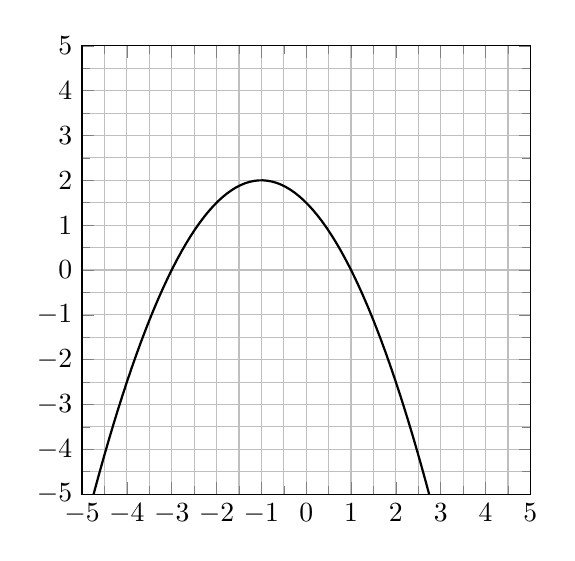
\begin{tikzpicture}[scale=1]
\begin{axis}[
	grid=both,
	unit vector ratio*=1 1,
	ymin=-5,
	ymax=5,
	xmax=5,
	xmin=-5,
	xtick={-5,-4,...,5},
	ytick={-5,-4,...,5}, 
	minor tick num=1
    ]
\addplot[thick, samples=100]   {(-(x+1)^2+4)/2};
\end{axis}
\end{tikzpicture}
\end{document}